%\newpage
\section{System Perspective}
\subsection{Design and Architecture}
\subsubsection*{Program Architecture}
\begin{figure}[H]
  \centering
  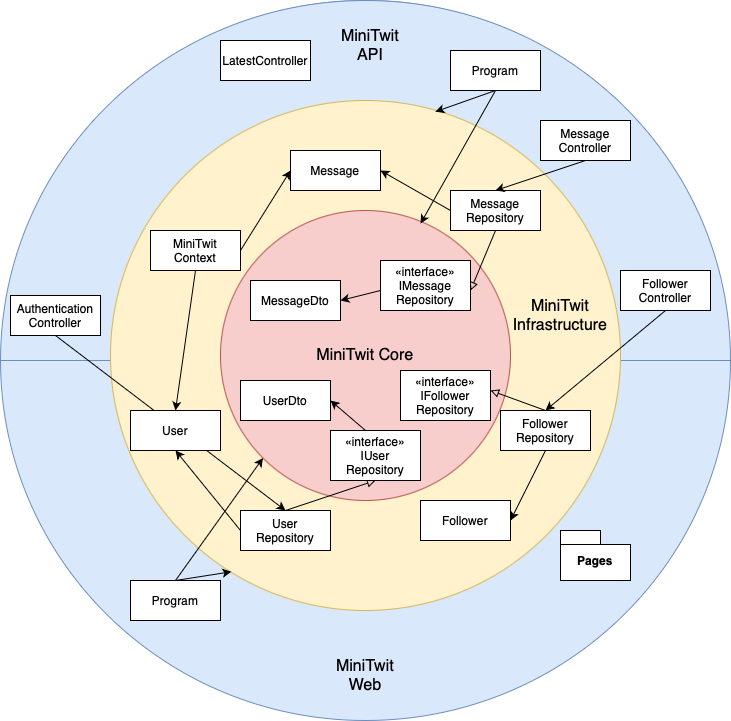
\includegraphics[width=0.75\linewidth]{Images/onion_architecture.png}
  \caption{Figure showing the architecture of our program.}
    \label{fig:onion}
\end{figure}

\subsubsection*{System Infrastructure}
\begin{figure}[H]
  \centering
  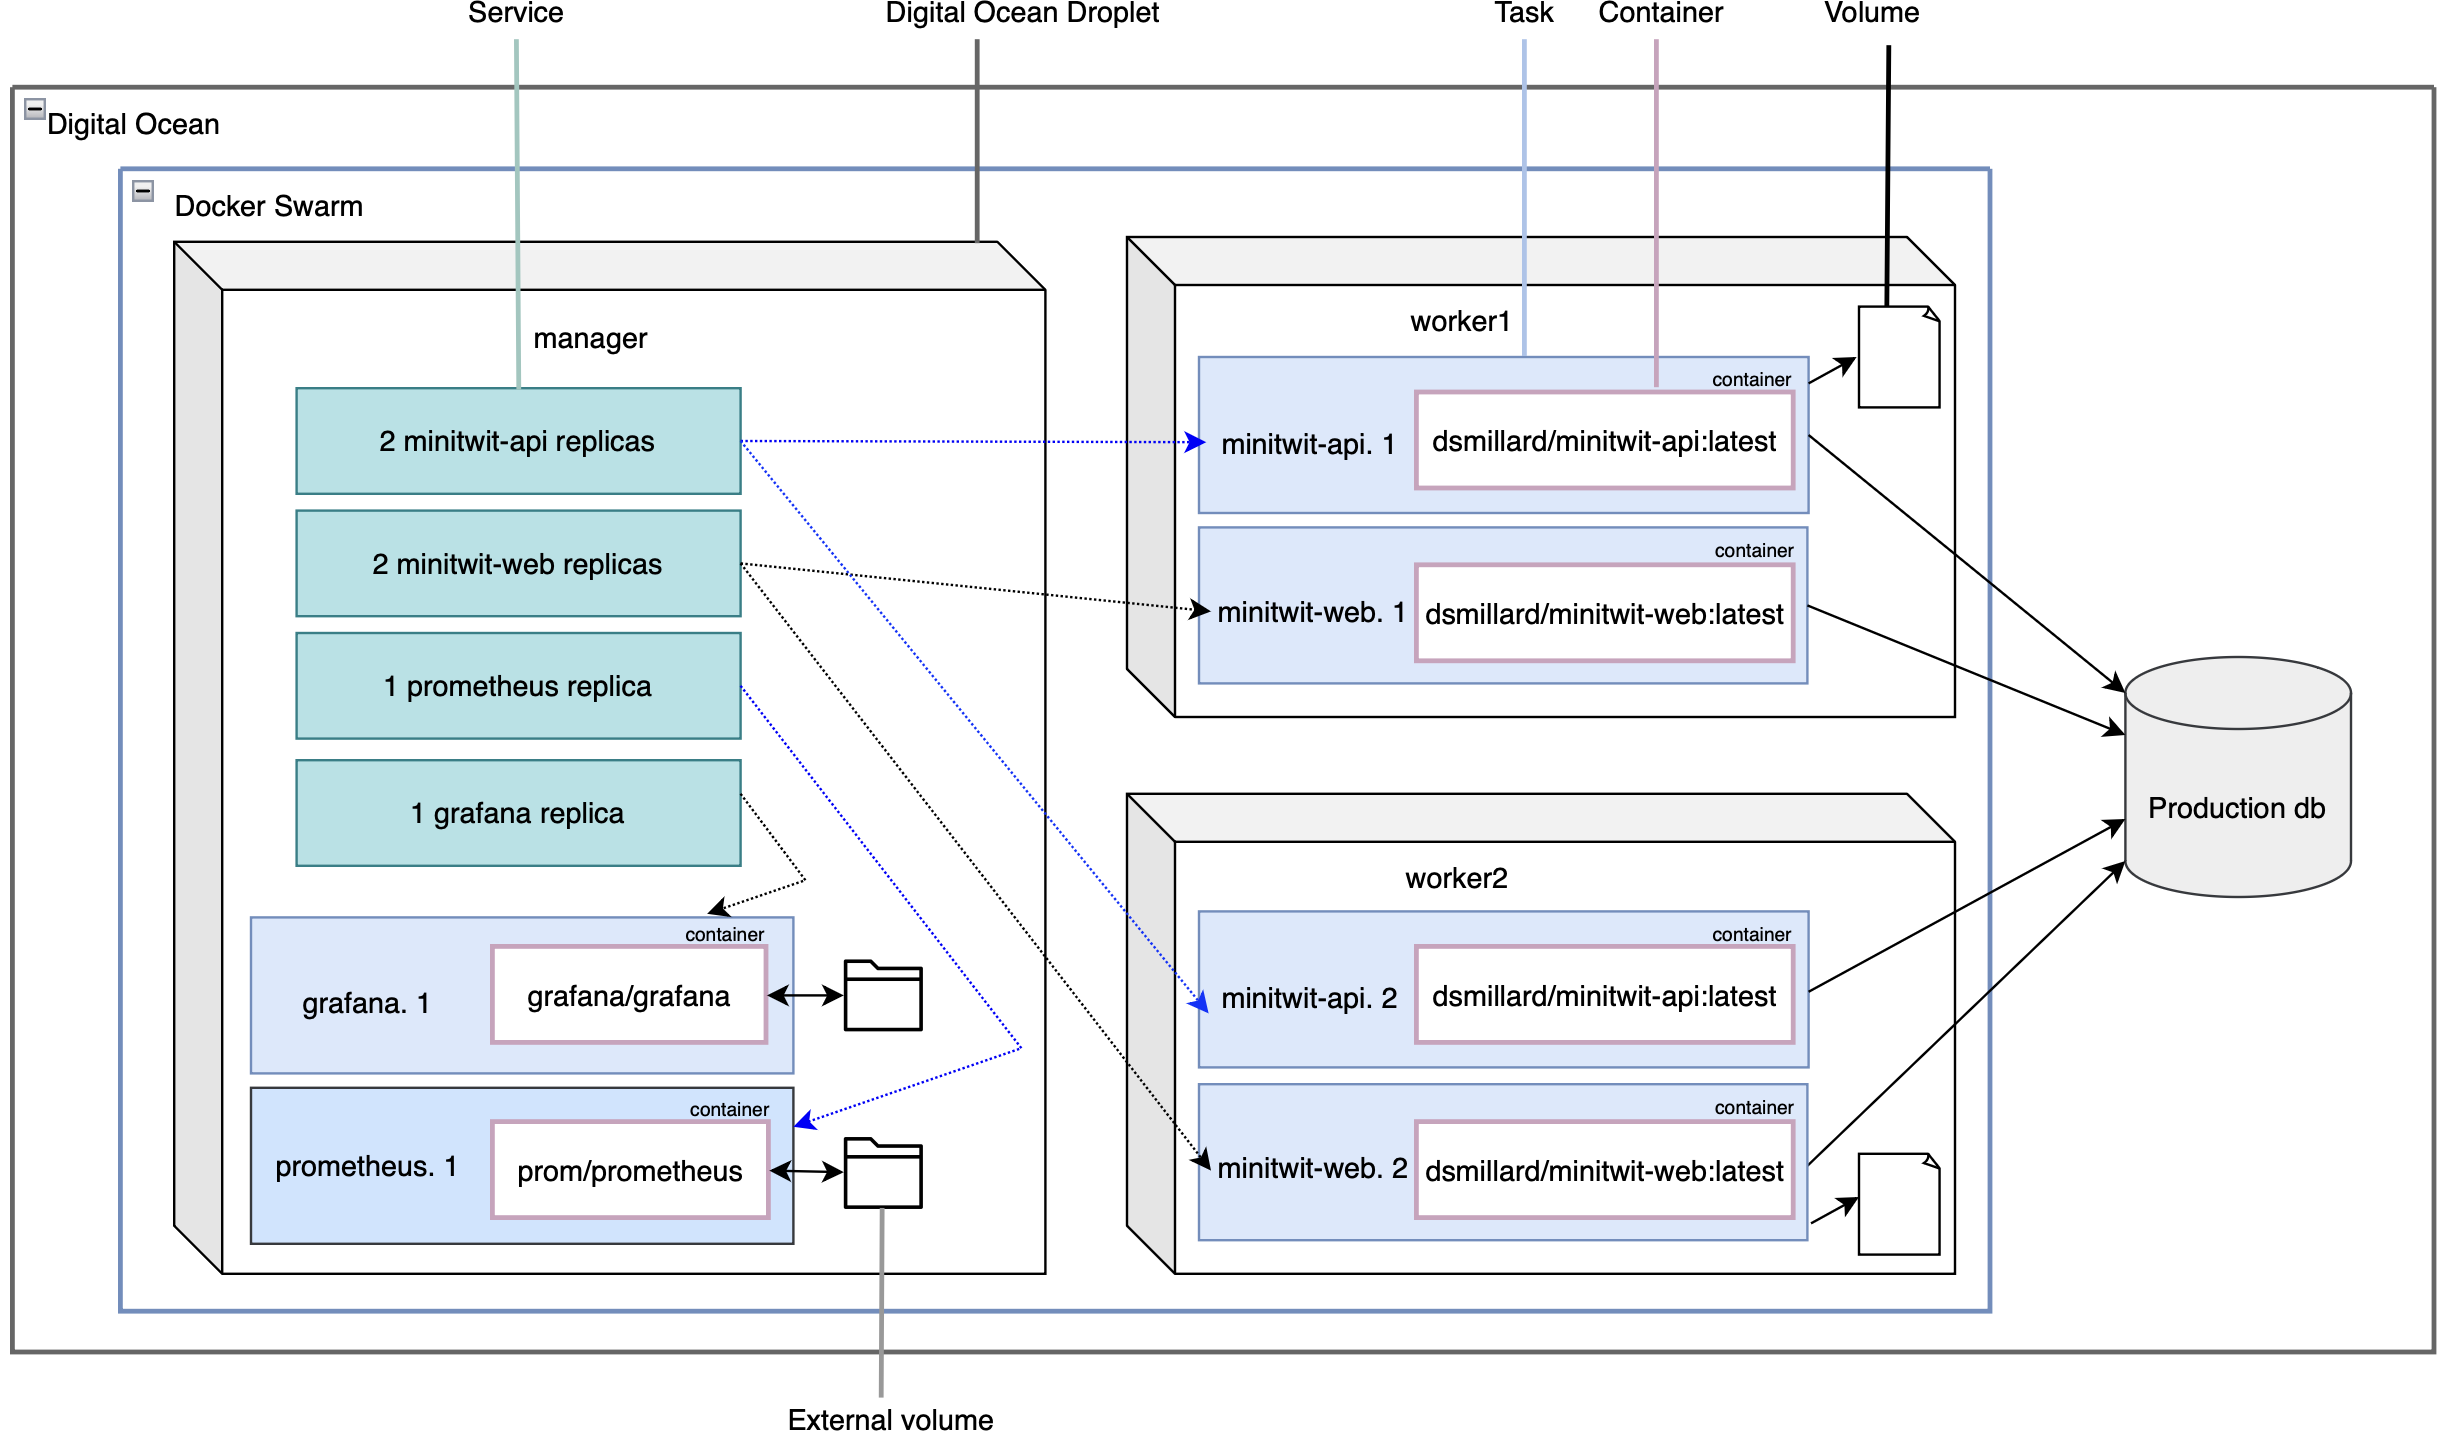
\includegraphics[width=\textwidth]{Images/docker_swarm.png}
  \caption{Overview of our system infrastructure.}
  \label{fig:dashboard}
\end{figure}

The system has 3 droplets; a manager and 2 worker nodes that form the application. The manager hosts the prometheus- and grafana-application, and the workers host the web- and api-application. The database is a managed database hosted on DigitalOcean.

\subsubsection*{Interaction of Subsystems}

\begin{figure}[H]
  \centering
  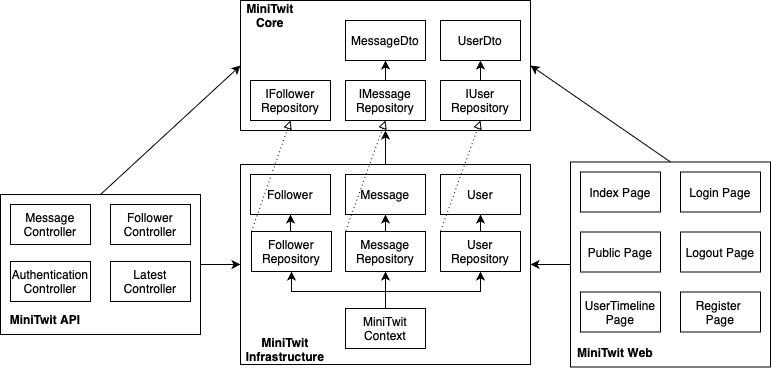
\includegraphics[width=\textwidth]{Images/interaction_of_subsystems.png}
  \caption{Overview of how our subsystems interact with eachother.}
  \label{fig:interaction_of_subsystems}
\end{figure}

Core is the smallest abstraction of our application. It only holds the data-transfer-objects and the interfaces for our repositories. Then comes the infrastructure that implements the interfaces from the Core and is the layer that is responsible for how we query the database. The API- and Web-application is the front of the application. They use the infrastructure to query the database and then either give something back to the user (API) or show the user something (Web).

\subsubsection*{Example of Interaction - API}

\begin{figure}[H]
  \centering
  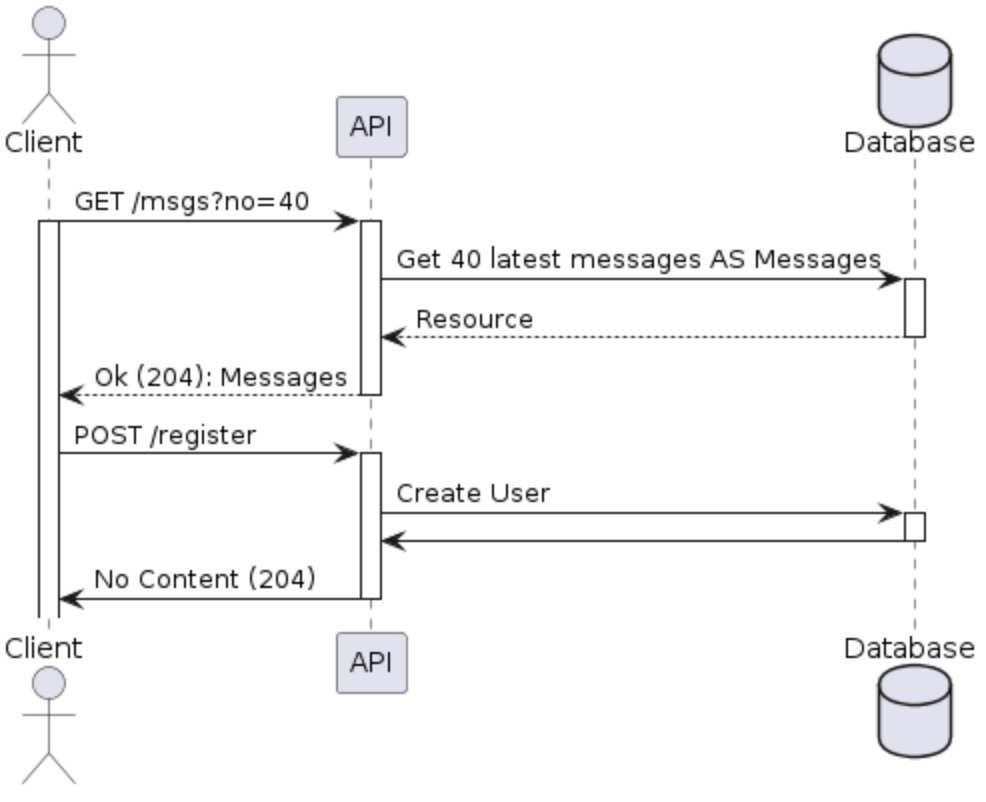
\includegraphics[width=0.75\linewidth]{Images/example_of_interaction.png}
  \caption{Example showing 2 interactions to the API; getting messages and registering a user.}
  \label{fig:example_interaction}
\end{figure}

\subsection[Dependencies \& Tools]{Dependencies \& Tools\footnote{All version numbers are as of 23/5-24}}

Operating System
\begin{itemize}
    \item Ubuntu 22.04 (LTS) x64
\end{itemize}

Development Environment
\begin{itemize}
    \item .NET SDK 8.0
\end{itemize}

Containerization
\begin{itemize}
    \item Docker v24.0.5
\end{itemize}

Database
\begin{itemize}
    \item PostgreSQL 16
\end{itemize}

Cloud Infrastructure:
\begin{itemize}
    \item \textbf{DigitalOcean} Used for hosting our application and managed databases.
\end{itemize}

Docker images:
\begin{itemize}
    \item \textbf{mcr.microsoft.com/dotnet/sdk:8.0}: Image containing the entire .NET SDK used for building the application. This image is currently also being deployed.
    \item \textbf{prom/prometheus@2.52.0}: Image containing a Prometheus instance configured by a .yml file.
    \item \textbf{grafana/grafana@10.1.10-ubuntu}: Image containing a Grafana instance configurable through a UI.
\end{itemize}

NuGet-packages:
\begin{itemize}
    \item \textbf{Npgsql.EntityFrameworkCore.PostgreSQL v8.0.2}: Entity Framework Core provider for PostgreSQL enabling interaction with PostgreSQL databases
    \item \textbf{prometheus-net.AspNetCore v8.2.1}: .NET library for instrumenting applications and exporting metrics to Prometheus.
    \item \textbf{Swashbuckle.AspNetCore v6.4.0}: Swagger tooling for generating Swagger UI for API endpoints, making them easier to test.
\end{itemize}


\subsection{Current State of The System}

\begin{figure}[H]
  \centering
  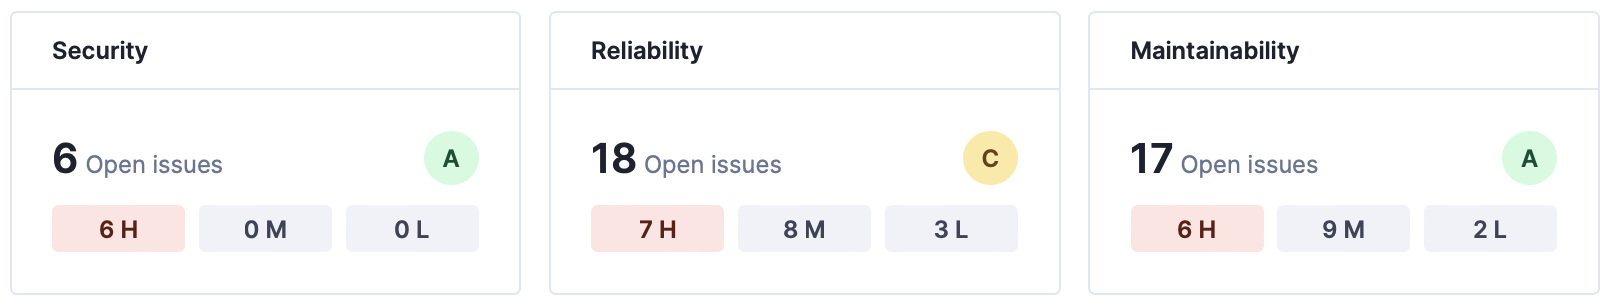
\includegraphics[width=\textwidth]{Images/sonarqube_stats.png}
  \caption{Latest summary from SonarQube showing our security-, reliability-, and maintainability-issues.}
  \label{fig:sonarqube_stats}
\end{figure}

\textbf{Security}: relates to us not checking if the model state is valid when using controller actions. \\
\textbf{Reliability}: relates to some async-problems, frontend-problems, and one unreachable code-problem. \\
\textbf{Maintainability}: relates to commented out code and some related to the tests file provided to us.

\begin{figure}[H]
  \centering
  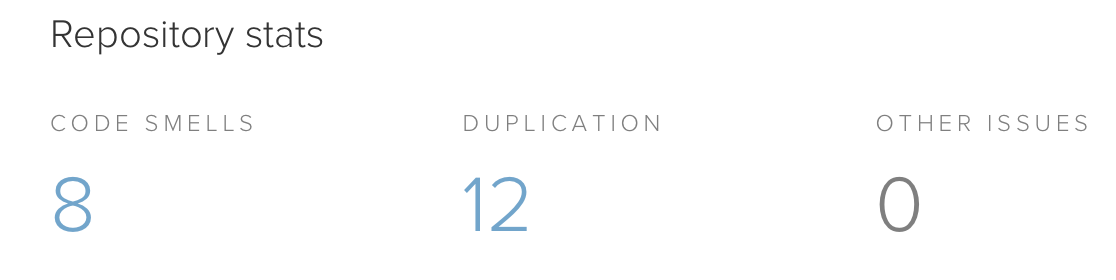
\includegraphics[width=\textwidth]{Images/codeclimate_stats.png}
  \caption{Latest summary from Code Climate showing our code smells and duplication issues.}
  \label{fig:codeclimate_stats}
\end{figure}

\textbf{Code Smells}: relates to some methods having more than 35 lines, one method having more than 4 arguments and some methods having too many return-statements. \\
\textbf{Duplication}: relates to some code-blocks showing up more than once.

\begin{figure}[H]
  \centering
  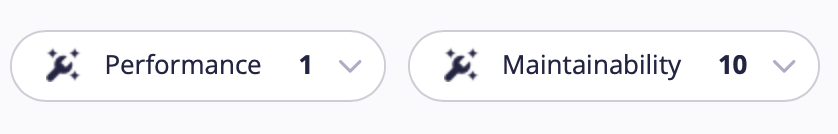
\includegraphics[width=\textwidth]{Images/codefactor_stats.png}
  \caption{Latest summary from CodeFactor showing our performance- and maintainability-issues.}
  \label{fig:codefactor_stats}
\end{figure}

\textbf{Performance}: relates to us allocating an array with zero-length. \\
\textbf{Maintainability}: relates to us having empty lines and some closing braces being preceded by a blank line.